\chapter{Introduction/序論}
\label{chap_Introduction}

Introduction/序論

\section{Review}
先行研究.

\begin{figure} % 特に強い理由がない限り、[htbp]のような指定はしないでください。
  \centering
%  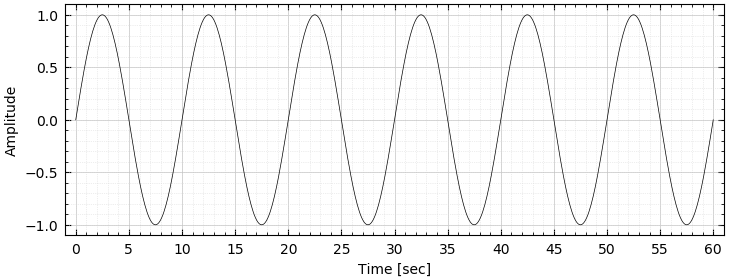
\includegraphics[width=4.9cm]{./figs/sin.png}
  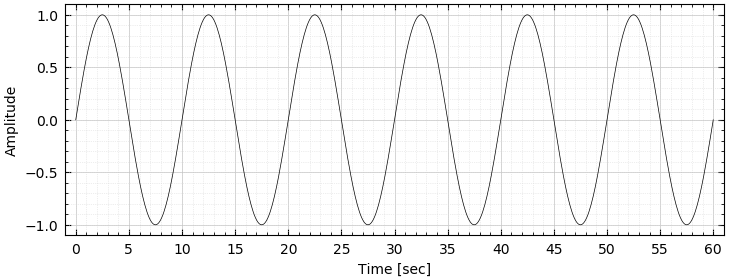
\includegraphics[width=15cm]{./figs/sin.png}
  \caption{
    Sin 波.区間 [0, 60] に発生している.図の説明は,「名詞句.文章.」の順番に説明するとよい.
    ここでは PNG 画像を貼り付けているが,pdf 等のベクトル図を貼り付けると,
    描画も印刷も格段に綺麗になる.pdf 形式でのグラフプロットは,Matplotlib の出力する拡張子を pdf に置き換えるだけである.
    なお,本画像の出典は \citep{ADMIS2018} であり,一部加工している.
  }
  \label{fig_ADMIS2018}
\end{figure}

\section{Purpose}
研究目的.

